\documentclass{article}
\usepackage{amsmath}
\usepackage{hyperref}
\usepackage{url}
\usepackage{amssymb}
\usepackage{graphicx}
\usepackage{float}
\usepackage{bm}
\usepackage[top=2cm]{geometry}
\renewcommand{\thesubsubsection}{\thesubsection\ \alph{subsubsection})}

\title{Deep Learning - Homework 1}
\author{99222 - Frederico Silva, 99326 - Sebastião Carvalho}
\date{\today}

\begin{document}

\maketitle

\tableofcontents

\section{Question 1}

\subsection{Question 1.1}

\subsection{Question 1.2}

\subsection{Question 1.3}

\subsection{Question 1.4}

\section{Question 2}

\subsection{Question 2.1}
After running the code, the best configuration was for the learning rate of 0.01.
The following plots were generated:

\begin{figure}[H]
    \centering
    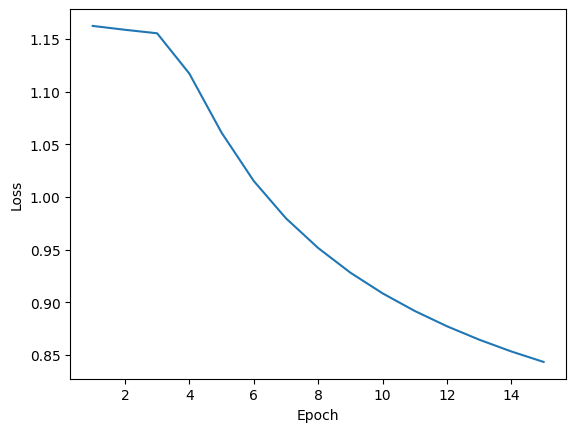
\includegraphics[width=0.8\textwidth]{plots/CNN-training-loss-0.01-0.7-0-sgd-False.png}
    \caption{Training loss for $\eta=0.01$}
    \label{fig:2.1-training_loss}
\end{figure}

\begin{figure}[H]
    \centering
    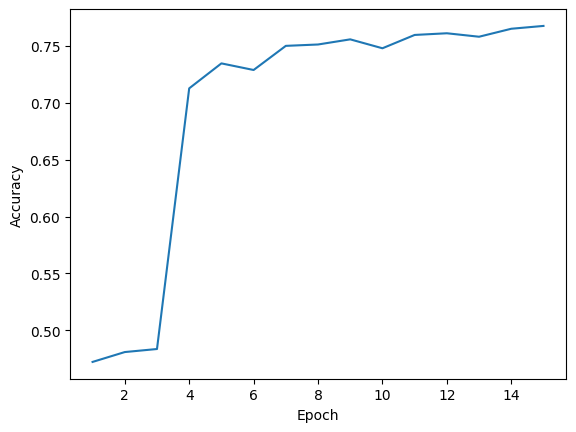
\includegraphics[width=0.8\textwidth]{plots/CNN-validation-accuracy-0.01-0.7-0-sgd-False.png}
    \caption{Validation accuracy for $\eta=0.01$}
    \label{fig:2.1-validation_accuracy}
\end{figure}

The final test accuracy was 0.8280.

\subsection{Question 2.2}
The performance of this network was slightly worse than the previous one, 
having achieved a final test accuracy of 0.8147.

\subsection{Question 2.3}
Both network present the same number of parameters, 224892.
The difference in performance between the two networks, resides in the use 
of max pooling layers. Max pooling can help the network focusing on the most
important features, making the network more robust to small changes in the
input. Furthermore, max pooling can also help with overfitting. In our case, 
the use of max pooling layers helped the network to achieve a better test 
accuracy results.

\section{Question 3}

\subsection{Question 3.1}

\subsection{Question 3.2}

\subsection{Question 3.3}

\subsection{Question 3.4}

\section{Credits}

\section{Sources}

\begin{itemize}
    \item \href{https://www.educative.io/answers/what-is-a-max-pooling-layer-in-cnn}{What is a max pooling layer in CNN?}
\end{itemize}

\end{document}